\documentclass[11pt, a4paper, leqno]{article}
\usepackage{a4wide}
\usepackage[T1]{fontenc}
\usepackage[utf8]{inputenc}
\usepackage{float, afterpage, rotating, graphicx}
\usepackage{epstopdf}
\usepackage{longtable, booktabs, tabularx}
\usepackage{fancyvrb, moreverb, relsize}
\usepackage{eurosym, calc, chngcntr}
\usepackage{amsmath, amssymb, amsfonts, amsthm, bm}
\usepackage{caption}
\usepackage{mdwlist}
\usepackage{xfrac}
\usepackage{setspace}
\usepackage{xcolor}

\usepackage[unicode=true]{hyperref}
\hypersetup{
    colorlinks=true,
    linkcolor=black,
    anchorcolor=black,
    citecolor=black,
    filecolor=black,
    menucolor=black,
    runcolor=black,
    urlcolor=black
}


\widowpenalty=10000
\clubpenalty=10000

\setlength{\parskip}{1ex}
\setlength{\parindent}{0ex}
\setstretch{1.5}


\begin{document}
\textbf{Empirical -- Monte Carlo Simulation}
\begin{enumerate}
\item Data generation
\item Definition of ichimura's and Klein and Spady's estimation methods
\item GridSearch: the way to choose an estimate
\item Definition of trimming function: data regularization
\item Bandwidth selection


\end{enumerate}
\section{Data Generation}
The baseline scenario of empirical monte carlo simulation is designed following Ichimura (1993): 
\begin{itemize}
\item sample size is 250;
\item the semiparametric single index model is specified as binary choice model such that estimation efficiency of Ichimura's method can be compared with that of Klein and Spady's method;
\item exogenous vector of variables contains two components and both are independently generated following standard normal distribution;
\item when constructing single index, parameter of the first exogenous component is normalized to 1 to satisty local normalization restriction of identification, and true value for the second parameter is set to -2;
\item preassume standard normal distribution for error distribution.
\end{itemize}
To summarize, the designed baseline function is
\begin{equation*}
y_i = I(x_{1i} - 2x_{2i} > \epsilon_i).
\end{equation*}

\section{Definition of Estimation Function} 
Following steps are taken to characterize ichimura's leave-one-out Nadaraya Watson estimator and Klein and Spady's maximum likelihood estimator:
\begin{enumerate}
\item define in both a fourth order Gaussian kernel function in order to achieve the kernel order requirment for Klein and Spady's method;
\item define a leave-one-out estimator function which returns the leave-one-out kernel estimator;
\item for Ichimura's method, define the objective function which minimizes sum of squared error, substituted with the differenct between true $y_i$ and the estimated value from last step; for Klein and Spady's method, define the objective function as the sum of estimated loglikelihood for occurance of true $y_i$s; 
\item note that the true value for $\beta_2$ is unknown, a list of possible candidates for vector $(1,\beta_2)$ are substituted into the defined objective function one after another, and the best candidate will be thereafter discovered. This is the idea behind GridSearch.
 
\end{enumerate}

\section{A Comparison between GridSearch and NLS}

\section{Definition of Data Trimming}

\section{Bandwidth Selection}

\section{A Result Comparison between Original Functions and Using NP Package}
($n = 250, m = 1000$)

\begin{table}[H]
\caption {Mean Squared Error Comparison} \label{tab:mean squared error}
\begin{tabular}{l r r}

\toprule
\textbf{method} & \textbf{NP Package} & \textbf{Original Functions} \tabularnewline\midrule
(standard normal distribution for $x_1$, $x_2$, $\epsilon$) & &
\tabularnewline
Ichimura & 0.00363 & 0.000260 \tabularnewline
Klein and Spady & 0.00416 & 0.000121 \tabularnewline

\bottomrule
\end{tabular}
\end{table}

\begin{figure}[h!]
  \caption{Plot of Estimates}
  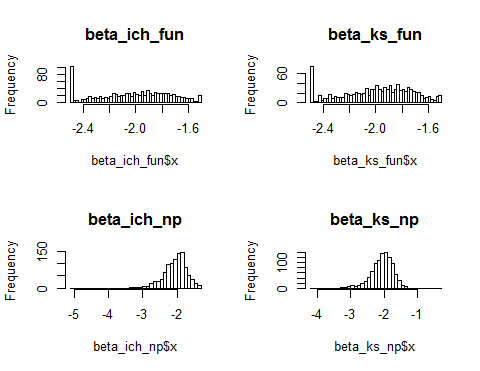
\includegraphics[width=\linewidth]{comparison_np_fun_plot.png}
 
  \label{fig:plot of estimates}
\end{figure}




\end{document}